\documentclass[twocolumn,10pt]{ltjsarticle}

\usepackage[top=20mm,bottom=20mm,left=25mm,right=25mm,columnsep=10mm]{geometry}
\usepackage[haranoaji,nfssonly]{luatexja-preset}
\usepackage{graphicx}
\usepackage{url}

\title{【調査】HTTPリクエスト/レスポンスによるマルウェア検知}
\author{山下 尚彦}
\date{\today}

\begin{document}
\maketitle

\section{はじめに}
昨今のサイバー攻撃は巧妙化しておりa, マルウェア感染を未然に防ぐことは困難となっている. 
なぜなら, 特定の組織やターゲットの機密情報を窃取する標的型攻撃が盛んになり, それとともに
攻撃が高度化・複雑化しているからである. 独立行政法人情報処理推進機構(IPA)によると, 
こういった高度な標的型攻撃は以下の7つの段階で構成されている\cite{IPA2014高度標的型攻撃}. 

\begin{description}
    \item[計画立案]~\\
    攻撃対象の調査・決定する

    \item[攻撃準備]~\\
    C2サーバを用意するなどの攻撃の準備をする 

    \item[初期侵入]~\\
    標的型メール, 水飲み場型攻撃などによって対象のネットワークに侵入を行う. 
    これらの攻撃者の行動はファイアウォールやアンチウイルスソフトウェア, 侵入検知システムでも完全には防ぐことはできない. 
    
    \item[基盤構築]~\\
    C2サーバとのバックドア通信を構築し, 感染端末が司令を受け取れるようにする

    \item[内部調査]~\\
    他の端末への侵入などによって対象となるネットワークの情報を調査する. 

    \item[目的遂行]~\\
    機密情報の窃取やシステムの破壊活動を行う. 

    \item[再侵入]~\\ 
    初期侵入時に利用した脆弱性や攻撃者が設置したバックドアから再び侵入し, 
    \textbf{内部調査}や\textbf{目的遂行}を繰り返す
\end{description}

また, 従来のマルウェアはC2サーバとの通信にIRCや独自のプロトコルを利用するため, ファイアウォールやプロキシ, 
トラフィックデータやログデータなどから振る舞いを学習させて検知するアノマリ検知によってその通信を遮断することは
比較的容易であった. しかし, 一般的な業務で頻繁に使用されているHTTPプロトコルを用いてC2サーバと通信を行う
高度なマルウェアの登場も検知を回避される要因となっている. \par
そこで, 小川らはトラフィックデータから取得したHTTPリクエストおよびHTTPレスポンス情報から特徴量を抽出し, 
Support Vector Machine(SVM)によって2値判定を行うことで検知する手法を提案した\cite{小川秀貴2016リクエスト間隔}. 
実験の結果, マルウェア感染由来のHTTPトラフィックの検知において高精度で検知することができ, 
またその見逃し率も低いという結果が出た. 

\section{提案手法}
前述したとおり, 小川らは正常な通信とマルウェア感染時の通信のリクエストの間隔とレスポンスのボディサイズから特徴量を抽出し, 
SVMによって2値判定を行うことでマルウェア感染由来のHTTPトラフィックの検知を目指す. 
関連研究では, レスポンスのボディ自体を参照するためプライバシーの観点から課題が存在したが, この手法はボディサイズのみ
着目するためプライバシーの保護に優位性があるとしている. \par
以下に示す手順によって識別機に学習させる. 

\begin{enumerate}
    \item \textbf{リクエスト/レスポンスのペアと構成}\\
    トラフィックデータからHTTPトラフィックを抽出し, さらにリクエスト時間, リクエストの送信元IPアドレス, 
    リクエストの送信先IPアドレス, レスポンスのボディサイズを抽出し, リクエストとレスポンスの情報をペアにする

    \item \textbf{通信ホストごとにペアを分割}\\
    マルウェア感染によってある通信先との間でトラフィックが発生しても, その他の通信先との間で正常なトラフィックが
    多く発生した場合, 抽出する特徴量が正常トラフィックの影響を大きく受けてしまう可能性があるため通信ホストごとに分割する

    \item \textbf{特徴ベクトルの抽出}\\
    以下のように通信ホストペアごとに分割した HTTP リクエスト/レス ポンスペアから,特徴ベクトルを抽出する. 
    \begin{enumerate}
        \item 通信ホスト毎に分割したHTTPリクエスト/レスポンスペアからリクエスト間隔および
        レスポンスボディサイズのリストを抽出する

        \item 抽出したリクエスト間隔及びレスポンスサイズを昇順にソートする

        \item ソート済みのリクエスト間隔及びレスポンスのボディサイズのリストからそれぞれ, 
        "最小値, 25パーセンタイル値, 中央値, 75パーセンタイル値, 最大値, 平均値, 標準偏差"の14個の特徴量を抽出
    \end{enumerate}

    \item \textbf{正規化}\\
    特徴量間でスケールが大きく異なる場合が起こりうるので, 平均0, 分散1となるようにデータセットから抽出した
    特徴量データの, 各特徴ベクトルの各値について平均値及び標準偏差を求めて個別に正規化する
\end{enumerate}

\section{実験}
小川らは正常/感染トラフィックのデータをあわせた2945個のデータセットをランダムに5分割, 各々のデータをテストデータとし, 
残りのデータを学習データとした評価実験を5回実施した. 
実験に使用したデータセットは, 正常/感染トラフィックのうち通信ホストペアでHTTPリクエストが5個以上存在し, 
特徴量を抽出できたものそれぞれ2378個と568個を使用した. 評価方法には, 数に偏りがあっても評価できる\textbf{Precision}と
\textbf{Recall}を用いた. それぞれの評価式が以下の\textbf{式\ref{eq:precision_n}}から\textbf{式\ref{eq:recall_p}}である. 

\begin{equation}
    \label{eq:precision_n}
    Precision_N = \frac{TN}{TN+FN}
\end{equation}

\begin{equation}
    \label{eq:precision_p}
    Precision_P = \frac{TP}{TP+FP}
\end{equation}

\begin{equation}
    \label{eq:recall_n}
    Recall_N = \frac{TN}{TN+FP}
\end{equation}

\begin{equation}
    \label{eq:recall_p}
    Recall_P = \frac{TP}{TP+FN}
\end{equation}

\begin{description}
    \item[$Precision_N$]~\\
    正常データと判定したデータの中で正しく正常と判定できた割合を示す
    \item[$Precision_P$]~\\
    感染と判定した中で正しく感染と判定で来た割合を示す
    \item[$Recall_N$]~\\
    正常データの中で正しく正常データと判定できた割合を示す
    \item[$Recall_P$]~\\
    感染データの中で正しく感染と判定できた割合を示す
    \item[$True Positive(TP)$]~\\
    実際は感染由来の通信であるものを正しく感染と判定したもの
    \item[$False Positive(FP)$]~\\
    実際は正常であるが予測では誤って感染と判定したもの
    \item[$True Negative(TN)$]~\\
    実際は感染であるものの正しく正常と判定したもの
    \item[$False Negative(FN)$]~\\
    実際は感染であるものの誤って正常と判定したもの
\end{description}

\section{実験結果}
実験を行った結果, 算出されたPrecisionとRecallを\textbf{表\ref{table:result}}に示す. 
$Precision_N$および$Precision_P$について, 正常と判定したもののうち96\%が正常であると正しく判定でき, 
感染と判定したものについては, 93\%が正しく判定できているため, 誤判定は少ないと言える. 
また, $Recall_N$や$Recall_P$について, すべての正常データのうち98\%は正しく判定できており, 
すべての感染データのうち85\%は正しく判定できているため, 見逃しは少ないと言える. 

\begin{table}[htb]
    \caption{実験結果}
    \label{table:result}
    \centering
    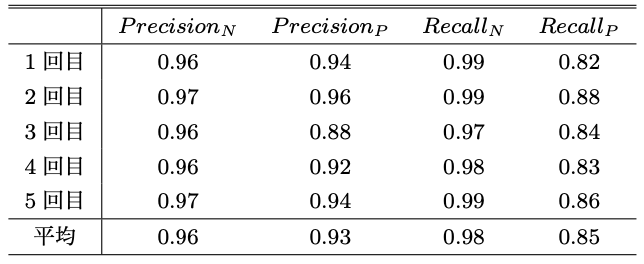
\includegraphics[width=6cm]{images/【調査】HTTPリクエスト,レスポンスによるマルウェア検知/result.png}
\end{table}

\section{おわりに}
従来の研究のように, マルウェア感染由来の通信が発生している同一のタイムスロットで正常通信が多く発生している場合, 
抽出した特徴量に対してのマルウェア感染由来の通信の影響は弱まるという課題があった. 
そこで小川らは, HTTPリクエストとそれに対応したHTTPレスポンスのペアを通信ホストごとに分割して特徴量を抽出することで, 
同一タイムスロット内の正常な通信がどれだけ多く発生しても, 抽出量に影響を及ぼさない手法を提案した. \par
正常な通信とマルウェア感染時の通信のデータをあわせたデータセットを分割して学習と判定を行い, この手法の実験を行った. 
その結果, 誤判定や見逃しは少なかった. \par
私の研究では, Lomb-Scargleピリオドグラムという手法を用いて, トラフィックデータのHTTPリクエストの間隔から
送信元IPアドレスと送信先IPアドレスの通信間で周期性があるかどうかを判定し, ボットとC2サーバの通信を検知する. 
しかし, 現状では周期的に通信を行っているIPアドレスのペアを検知することはできるが, 
それが正常な通信かマルウェアの感染による通信なのかを区別することができないため, 小川らの検知手法と組み合わせることで
より精度の高い検知ができるのではないかと考えられる. 


\bibliographystyle{junsrt}
\bibliography{DB}
\end{document}
